% !TEX root = ../OT4ML.tex


%%%%%%%%%%%%%%%%%%%%%%%%%%%%%%%%%%%%%%%%%%%%%%%%%%%%%%%%%%%%%%%%%%%%%%%%%%%
%%%%%%%%%%%%%%%%%%%%%%%%%%%%%%%%%%%%%%%%%%%%%%%%%%%%%%%%%%%%%%%%%%%%%%%%%%%
%%%%%%%%%%%%%%%%%%%%%%%%%%%%%%%%%%%%%%%%%%%%%%%%%%%%%%%%%%%%%%%%%%%%%%%%%%%
\section{Sinkhorn}
\label{sec-sinkhorn}

Entropic regularization makes optimal transport smooth, strictly convex and scalable. This section explains why adding entropy produces matrix scaling, how Sinkhorn iterations enforce the marginals, and why this simple algorithm became the computational workhorse of OT. The presentation connects the older matrix-scaling literature~\cite{Sinkhorn64,SinkhornKnopp67,Sinkhorn67} with modern entropic OT~\cite{CuturiSinkhorn,peyre2019computational}.

%%%%%%%%%%%%%%%%%%%%%%%%%%%%%%%%%%%%%%%%%%%%%%%%%%%%%%%%%%%%%%%%%%%%%%%%%%%
\subsection{Entropic Regularization for Discrete Measures}
\label{sec-entropic-discrete}

Entropy turns a possibly non-unique linear program into a unique smooth problem. The price is bias, but the reward is differentiability and fast scaling algorithms.

%%%%%
\paragraph{Entropic Regularization for Discrete Measures.}


The idea of the entropic regularization of optimal transport is to use the Shannon-Boltzmann entropy
\eq{
	\HD(\P) \eqdef -\sum_{i,j} \P_{i,j} \log(\P_{i,j}),
}
with the convention $0 \log(0)=0$
as a regularizing function to obtain approximate solutions to the original transport problem~\eqref{eq-kanto-discr}
\eql{\label{eq-regularized-discr}
	\MKD_\C^\epsilon(\a,\b) \eqdef
	\umin{\P \in \CouplingsD(\a,\b)}
		\dotp{\P}{\C} - \epsilon \HD(\P).
}

\begin{prop}[Existence and uniqueness of entropic OT]\label{prop-entropic-unique}
	Assume that $\a,\b$ are probability histograms and that $\C$ is finite. For every $\epsilon>0$, problem~\eqref{eq-regularized-discr} admits a unique minimizer. If all entries of $\a$ and $\b$ are positive, then this minimizer is positive on every entry.
\end{prop}

\begin{proof}
	The transport polytope $\CouplingsD(\a,\b)$ is non-empty and compact, and the objective is continuous on it with the convention $0\log0=0$, so a minimizer exists. On the relative interior of the polytope,
	\[
		-\partial^2 \HD(\P)=\diag(1/\P_{i,j})
	\]
	is positive definite on every non-zero feasible direction. Hence $-\HD$ is strictly convex on the polytope and $\dotp{\P}{\C}-\epsilon\HD(\P)$ is strictly convex, which implies uniqueness.

	If $\a_i,\b_j>0$ and a minimizer had $\P_{i,j}=0$, then for small $t>0$ the perturbation $\P_t=(1-t)\P+t\,\a\otimes\b$ remains feasible. The directional derivative of the entropic part at $t=0$ is $-\infty$ because the derivative of $r\log r$ at $0$ is $-\infty$ along a positive direction. Thus the objective decreases for small $t$, contradicting optimality. Therefore the minimizer is strictly positive.
\end{proof}


%%%%%
\paragraph{Smoothing effect.}

By Proposition~\ref{prop-entropic-unique}, problem~\eqref{eq-regularized-discr} has a unique optimal solution.
%
This smoothing, beyond providing uniqueness, actually leads to $\MKD_\C^\epsilon(\a,\b)$ being a smooth function of $\a$, $\b$ and $\C$ whenever these variables stay in the relative interior of their domains. In finite dimension, this follows from strict convexity and the envelope theorem applied to the dual problem.
%
The effect of the entropy is to act as a barrier function for the positivity constraint. As we will show later, this forces the solution $\P$ to be strictly positive on the support of $\a \otimes \b$. We will also show that as $\epsilon\to+\infty$, the solution satisfies $\P \to \a \otimes \b$.

\begin{figure}[H]
\centering
\begin{tabular}{@{}cccc@{}}
\small large $\epsilon$ &
\small medium $\epsilon$ &
\small small $\epsilon$ &
\small entropic path \\[-.15em]

\includegraphics[width=.21\linewidth]{figures/sinkhorn-entropy-lp-geometry/eps-large.pdf} &

\includegraphics[width=.21\linewidth]{figures/sinkhorn-entropy-lp-geometry/eps-medium.pdf} &

\includegraphics[width=.21\linewidth]{figures/sinkhorn-entropy-lp-geometry/eps-small.pdf} &

\includegraphics[width=.21\linewidth]{figures/sinkhorn-entropy-lp-geometry/path.pdf}
\end{tabular}
\caption{Entropic regularization of a linear objective on a two-dimensional face of the transport polytope. The gray lines are linear objective levels. The first three panels show the unique entropic minimizer for decreasing regularization strengths $\epsilon=1.10,0.35,0.095$; the last panel shows the continuous path traced by the minimizer as $\epsilon$ decreases. The entropy barrier keeps the solution in the relative interior for every $\epsilon>0$, while the path approaches the low-cost vertex.}
\label{fig:sinkhorn-entropy-lp-geometry}
\end{figure}


%%%%%%%%%%%%%%%%%%%%%%%%%%%%%%%%%%%%%%%%%%%%%%%%%%%%%%%%%%%%%%%%%%%%%%%%%%%
\subsection{Sinkhorn's Algorithm}


Sinkhorn's algorithm is alternating normalization of rows and columns. This subsection derives the scaling form of the optimizer and explains why each iteration only needs matrix-vector products.

The underlying matrix-scaling iteration has a long history, including iterative proportional fitting and the work of Sinkhorn and Knopp~\cite{Sinkhorn64,SinkhornKnopp67,Sinkhorn67}. Its modern role in OT was transformed by Cuturi's entropic formulation~\cite{CuturiSinkhorn}: the algorithm became a practical large-scale tool for machine learning, and also changed the way OT is viewed in ML, from a mostly geometric distance to a differentiable computational primitive.

The following proposition shows that the solution of~\eqref{eq-regularized-discr} has a specific form, which can be parameterized using $n+m$ variables. That parameterization is therefore essentially dual, in the sense that a coupling $\P$ in $\CouplingsD(\a,\b)$ has $nm$ variables but $n+m$ constraints.

\begin{prop}[Scaling form of entropic OT]\label{prop-regularized-primal}
$\P$ is the unique solution to~\eqref{eq-regularized-discr} if and only if there exists  $(\uD,\vD) \in \RR_+^n \times \RR_+^m$ such that
\eql{\label{eq-scaling-form}
	\foralls (i,j) \in \range{n} \times \range{m}, \quad \P_{i,j} = \uD_i \K_{i,j} \vD_j
		\qwhereq \K_{i,j} \eqdef e^{-\frac{\C_{i,j}}{\epsilon}},
}
and $\P \in \Couplings(\a,\b)$.
\end{prop}

	\begin{proof}
	Without loss of generality, we assume $\a_i,\b_j>0$ (otherwise, rows or columns with zero mass are fixed to zero and can be removed). By Proposition~\ref{prop-entropic-unique}, the minimizer is strictly positive on the remaining support.

	We can thus ignore the positivity constraint when introducing two dual variables $\fD\in\RR^n,\gD\in\RR^m$ for each marginal constraint so that the Lagrangian of~\eqref{eq-regularized-discr} reads
	\eq{\label{eq-sinkhorn-lagrangian}
		\Lag(\P,\fD,\gD)=
		\dotp{\P}{\C}
		+\epsilon\sum_{i,j}\P_{i,j}\log(\P_{i,j})
		+ \dotp{\fD}{\a - \P\ones_m}
		+ \dotp{\gD}{\b - \transp{\P}\ones_n}.
	}
Considering first-order conditions (where we ignore the positivity constraint as explained above), we have
$$
	\frac{\partial\Lag(\P,\fD,\gD)}{\partial \P_{i,j}}= \C_{i,j} + \epsilon (\log\pa{ \P_{i,j} }+1) - \fD_i -\gD_j = 0.
$$
which results, in an optimal $\P$ coupling of the regularized problem, in the expression
$\P_{i,j}=e^{\frac{\fD_i+\gD_j - \C_{i,j}}{\epsilon}-1}$
which can be rewritten in the form provided in the proposition using non-negative vectors $\uD_i \eqdef e^{\fD_i/\epsilon-1}$ and $\vD_j \eqdef e^{\gD_j/\epsilon}$.
\end{proof}

The factorization of the optimal solution exhibited in Equation~\eqref{eq-scaling-form} can be conveniently rewritten in matrix form as $\P=\diag(\uD)\K\diag(\vD)$.
%
$\uD,\vD$ must therefore satisfy the following nonlinear equations which correspond to the mass conservation constraints inherent to $\CouplingsD(\a,\b)$,
\eql{\label{eq-dualsinkhorn-constraints}
	\diag(\uD)\K\diag(\vD)\ones_m=\a,
	\qandq
	\diag(\vD)\K^\top \diag(\uD)\ones_n=\b,
}
These two equations can be further simplified, since $\diag(\vD)\ones_m$ is  $\vD$, and the multiplication of $\diag(\uD)$ times $\K \vD$ is
\eql{\label{eq-dualsinkhorn-constraints2}
	\uD \odot (\K \vD) = \a
	\qandq
	\vD \odot (\transp{\K}\uD) = \b
}
where $\odot$ corresponds to the entry-wise multiplication of vectors. This problem is known in the numerical analysis community as the matrix scaling problem (see~\cite{nemirovski1999complexity} and references therein).

The problem of normalizing a positive matrix $\K$ has a long history, from iterative proportional fitting in statistics and economics~\cite{kruithof,yule1912methods,Galichon-Entropic} to modern matrix balancing algorithms~\cite{ReviewSinkhorn,cohen2017matrix}.
%
The problem of normalizing a positive matrix $\K$ by diagonal scaling is well known, in particular when $n=m$ and $\a$ and $\b$ are uniform. This corresponds to diagonal scaling toward bistochasticity, which is a very old problem. The previous result shows that there is a unique such scaled matrix $\P$, thanks to the strong convexity of the regularized problem. The remaining question is how to compute this scaled matrix in practice. If some entries of $\K$ vanish (equivalently, if the cost matrix $\C$ can have infinite values), additional support conditions are needed; here we focus on the strictly positive case.


An intuitive way to try to solve these equations is to solve them iteratively, by modifying first $\uD$ so that it satisfies the left-hand side of Equation~\eqref{eq-dualsinkhorn-constraints2} and then $\vD$ to satisfy its right-hand side. These two updates define Sinkhorn's algorithm
\eql{\label{eq-sinkhorn}
	\itt{\uD} \eqdef \frac{\a}{\K \it{\vD}}
	\qandq
	\itt{\vD} \eqdef \frac{\b}{\transp{\K}\itt{\uD}},
}
initialized with an arbitrary positive vector, for instance $\init{\vD} = \ones_m$. The division operator used above between two vectors is to be understood entry-wise. Note that a different initialization will likely lead to a different solution for $\uD,\vD$, since $\uD,\vD$ are only defined up to a multiplicative constant (if $\uD,\vD$ satisfy \eqref{eq-dualsinkhorn-constraints} then so do $\lambda\uD,\vD/\lambda$ for any $\lambda>0$).
%
The alternating normalization can be read directly on the coupling matrix: a row update enforces the source marginal and generally perturbs the target marginal, while the next column update does the converse.

\begin{figure}[H]
\centering
\setlength{\tabcolsep}{1.5pt}
\begin{tabular}{@{}ccccc@{}}
\small initial $K$ &
\small row 1 &
\small column 1 &
\small row 2 &
\small column 2 \\[-.15em]

\includegraphics[width=.18\linewidth]{figures/sinkhorn-marginal-errors/initial.pdf} &

\includegraphics[width=.18\linewidth]{figures/sinkhorn-marginal-errors/row-1.pdf} &

\includegraphics[width=.18\linewidth]{figures/sinkhorn-marginal-errors/column-1.pdf} &

\includegraphics[width=.18\linewidth]{figures/sinkhorn-marginal-errors/row-2.pdf} &

\includegraphics[width=.18\linewidth]{figures/sinkhorn-marginal-errors/column-2.pdf}
\end{tabular}
\caption{Marginal constraints during Sinkhorn scaling on a twelve-bin one-dimensional problem. Violet circles represent the current coupling matrix; hollow side circles show the prescribed red row marginal and blue column marginal, while filled side circles show the current marginals. Row normalizations align the red marginal and leave a blue defect; column normalizations align the blue marginal and leave a red defect.}
\label{fig:sinkhorn-marginal-errors}
\end{figure}

The same alternating projection mechanism is clearer on a dense one-dimensional discretization, where the marginal defects appear as continuous side curves.

\begin{figure}[H]
\centering
\begin{tabular}{@{}cccc@{}}
\small initial $K$ &
\small after one row scaling &
\small after one column scaling &
\small after 12 cycles \\[-.15em]

\includegraphics[width=.22\linewidth]{figures/sinkhorn-continuous-marginal-scaling/initial.pdf} &

\includegraphics[width=.22\linewidth]{figures/sinkhorn-continuous-marginal-scaling/row-1.pdf} &

\includegraphics[width=.22\linewidth]{figures/sinkhorn-continuous-marginal-scaling/column-1.pdf} &

\includegraphics[width=.22\linewidth]{figures/sinkhorn-continuous-marginal-scaling/column-12.pdf}
\end{tabular}
\caption{Dense Sinkhorn scaling for one-dimensional Gaussian-mixture marginals. The grayscale matrix is the current coupling. The red and blue side curves are the prescribed source and target marginals, while the violet side curves are the current row and column sums. A row scaling makes the violet curve coincide with the red source marginal, a column scaling makes it coincide with the blue target marginal, and the alternation rapidly stabilizes both sides.}
\label{fig:sinkhorn-continuous-marginal-scaling}
\end{figure}

Once both marginals are nearly enforced, the coupling matrix itself stabilizes.

\begin{figure}[H]
\centering
\begin{tabular}{@{}ccccc@{}}
\small $k=0$ &
\small $k=1$ &
\small $k=3$ &
\small $k=12$ &
\small $k=60$ \\[-.15em]
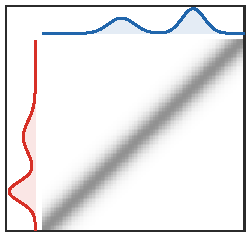
\includegraphics[width=.175\linewidth]{figures/sinkhorn-coupling-iterations/iter-0.pdf} &
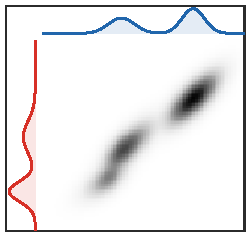
\includegraphics[width=.175\linewidth]{figures/sinkhorn-coupling-iterations/iter-1.pdf} &
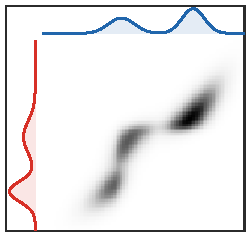
\includegraphics[width=.175\linewidth]{figures/sinkhorn-coupling-iterations/iter-3.pdf} &
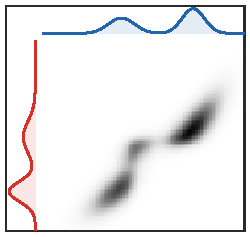
\includegraphics[width=.175\linewidth]{figures/sinkhorn-coupling-iterations/iter-12.pdf} &
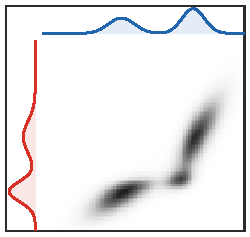
\includegraphics[width=.175\linewidth]{figures/sinkhorn-coupling-iterations/iter-60.pdf}
\end{tabular}
\caption{Coupling matrices along Sinkhorn iterations for the same one-dimensional setting as Figure~\ref{fig:sinkhorn-dual-potentials-epsilon}, with fixed $\epsilon=0.045$. The panels show the matrix after $k$ complete row-column scaling cycles and use a common grayscale normalization. The initial Gibbs kernel is a diagonal-like affinity matrix; scaling bends and reweights it until its row and column sums match the prescribed marginals.}
\label{fig:sinkhorn-coupling-iterations}
\end{figure}

The next paragraphs explain why these iterations converge.

\begin{figure}[ht]
\centering
\setlength{\tabcolsep}{2pt}
\begin{tabular}{@{}cccc@{}}
\small $k=0$ &
\small $k=1$ &
\small $k=3$ &
\small $k=12$ \\[-.15em]

\includegraphics[width=.23\linewidth]{figures/sinkhorn-potentials-iterations/iter-0.pdf} &

\includegraphics[width=.23\linewidth]{figures/sinkhorn-potentials-iterations/iter-1.pdf} &

\includegraphics[width=.23\linewidth]{figures/sinkhorn-potentials-iterations/iter-3.pdf} &

\includegraphics[width=.23\linewidth]{figures/sinkhorn-potentials-iterations/iter-12.pdf}
\end{tabular}
\caption{KL-normalized Sinkhorn dual potentials along the scaling iteration for the same one-dimensional Gaussian-mixture setting as Figure~\ref{fig:sinkhorn-dual-potentials-epsilon}, with fixed regularization strength $\epsilon=0.045$. The faint red and blue silhouettes show the source and target histograms, and the red and blue curves are the logarithmic scaling potentials. All panels share the same axes, making stabilization visible.}
\label{fig:sinkhorn-potentials-iterations}
\end{figure}

Complexity bounds for Sinkhorn and comparisons with accelerated first-order methods are discussed in~\cite{altschuler2017near,pmlr-v80-dvurechensky18a,knight2008sinkhorn}.
%
A chief computational advantage of Sinkhorn's algorithm, besides its simplicity, is that the only expensive step is multiplication by the Gibbs kernel. Its complexity therefore scales like $Cnm$, where $C$ is the number of Sinkhorn iterations. Section~\ref{sec-convergence-dual} gives a more precise convergence statement: for a fixed regularization strength $\epsilon$, the entropic dual gap has an $O(1/k)$ bound with constants proportional to $1/\epsilon$, while Hilbert-metric arguments give eventual linear convergence when the Gibbs kernel is uniformly positive. To approximate the unregularized OT value to accuracy $\delta$, one must also balance the entropic bias, which is typically $O(\epsilon)$ in finite dimension. Choosing $\epsilon$ proportional to $\delta$ and solving the entropic problem to accuracy $O(\delta)$ leads to the familiar iteration scaling of order $1/\delta^2$ for the unregularized value, up to logarithmic and cost-range factors~\cite{altschuler2017near,pmlr-v80-dvurechensky18a}.

\begin{figure}[H]
\centering

\includegraphics[width=.50\linewidth]{figures/sinkhorn-linear-rate-epsilon/marginal-error.pdf}
\caption{Marginal violation along Sinkhorn half-steps for four values of $\epsilon$ on the same one-dimensional Gaussian-mixture problem. The plotted error is $\frac12(\|P_k\ones-\a\|_1+\|P_k^\top\ones-\b\|_1)$ on a logarithmic scale. For fixed positive $\epsilon$, the curves enter a linear regime; smaller $\epsilon$ gives a sharper transport geometry but a more peaked Gibbs kernel and slower scaling.}
\label{fig:sinkhorn-linear-rate-epsilon}
\end{figure}

In many applications, however, one does not need a highly accurate optimizer for the OT subproblem. Downstream performance is often tied more to the geometric bias of the discrepancy than to exact optimality. In such settings, $C$ is often moderate.
%
This should be contrasted with interior point methods, which also operate by introducing a barrier function of the form $-\sum_i \log(\P_{i,j})$. For a dense transportation linear program, these algorithms typically have worst-case complexity of order $O(n^6 \log(1/\delta))$ to reach accuracy $\delta$, up to problem-dependent conditioning factors.

The second crucial aspect of Sinkhorn is that matrix-vector multiplication streams extremely well on GPU. Even better, if one is interested in computing many OT problems with a fixed cost matrix $\C$, one can replace many matrix-vector multiplications with matrix-matrix multiplications, so that the computational gain can be substantial.

\begin{rem}[Separable Gaussian kernels on grids]\label{rem-sinkhorn-separable-gaussian}
	When the samples lie on a Cartesian grid and $c(x,y)=\norm{x-y}^2$, the Gibbs kernel is Gaussian and factorizes along coordinates. If the grid has $q$ points per axis in dimension $d$, so that $N=q^d$ grid points are used, then
	\[
		K(x,y)=\exp\!\left(-\frac{\norm{x-y}^2}{\epsilon}\right)
		=
		\prod_{\ell=1}^d
		\exp\!\left(-\frac{(x_\ell-y_\ell)^2}{\epsilon}\right).
	\]
	Multiplication by $K$ can therefore be applied by successively multiplying along each coordinate direction, equivalently by applying one-dimensional Gaussian kernel operators along the axes. On a periodic or sufficiently padded uniform grid these are literal discrete convolutions. A direct dense one-dimensional multiplication costs $O(q^2)$ on each of the $q^{d-1}$ coordinate lines, and this is repeated for $d$ axes. Hence one Sinkhorn half-step costs
	\[
		O(d\,q^{d+1})=O(d\,N^{1+1/d})
	\]
	instead of $O(N^2)$. With FFT-based or truncated Gaussian convolutions, the same separability can be pushed further, but the simple tensor-product estimate already explains why grid-based Sinkhorn can scale much better than a generic dense coupling.
\end{rem}


%%%%%%%%%%%%%%%%%%%%%%%%%%%%%%%%%%%%%%%%%%%%%%%%%%%%%%%%%%%%%%%%%%%%%%%%%%%
\subsection{Reformulation using relative entropy}

The KL formulation identifies Sinkhorn as a projection method. It also prepares the continuous and unbalanced settings, where a reference measure is essential.

A convenient tool to reformulate and ``normalize'' this discrete entropy (which is crucial to formulate a continuous version of the problem below) is to consider the relative entropy, also called the Kullback--Leibler divergence, which is defined as
\eql{\label{eq-kl-defn}
	\KLD(\P|\Q) \eqdef \sum_{i,j}  \P_{i,j} \log\pa{\frac{\P_{i,j}}{\Q_{i,j}}} - \P_{i,j} + \Q_{i,j}.
}
with the convention $0\log(0)=0$ and $\KLD(\P|\Q)=+\infty$ if there exists some $(i,j)$ such that $\Q_{i,j}=0$ but $\P_{i,j} \neq 0$.
%
For the specific case of comparing probability distributions, this further simplifies to
\eq{
	\KLD(\P|\Q) = \sum_{i,j}  \P_{i,j} \log\pa{\frac{\P_{i,j}}{\Q_{i,j}}}.
}
The Shannon-Boltzmann neg-entropy is obtained when considering $\Q=\ones_{n \times m}$, i.e.
\eq{
	\HD( \P ) = -\KLD(\P|\ones_{n \times m}).
}
$\KLD$ is a particular instance of both a $\phi$-divergence (as defined in Section~\ref{sec-phi-div}) and a Bregman divergence; up to standard affine rescalings, it is the canonical overlap between these two families. This special property is at the heart of the fact that this regularization leads to elegant algorithms and a tractable mathematical analysis.

\begin{prop}[Relative entropy is distance-like]\label{prop-kl-distance-like}
	Let $\P,\Q\in\RR_+^{n\times m}$ have the same total mass and assume $\Q_{i,j}>0$ on the support of $\P$. Then $\KLD(\P|\Q)\geq0$, with equality if and only if $\P=\Q$.
\end{prop}
\begin{proof}
	Write $\phi(s)=s\log s-s+1$. Convexity gives $\phi(s)\geq \phi(1)+\phi'(1)(s-1)=0$, and strict convexity gives equality only at $s=1$. Hence
	\[
		\KLD(\P|\Q)=\sum_{i,j}\Q_{i,j}\phi(\P_{i,j}/\Q_{i,j})\geq0,
	\]
	with equality only when $\P_{i,j}/\Q_{i,j}=1$ for all entries with $\Q_{i,j}>0$. The support convention rules out positive $\P$ where $\Q=0$, so equality is equivalent to $\P=\Q$.
\end{proof}

Equivalently, when $\P$ and $\Q$ have the same total mass, it reads
\eq{
	\KLD(\P|\Q) = \sum_{i,j}  \phi( \P_{i,j} / \Q_{i,j} ) \Q_{i,j}.
}
where $\phi(s)=s\log(s)$. For any convex $\phi$ such that $\phi(1)=0$, one has indeed by Jensen
\eq{
	\sum_{i,j}  \phi( \P_{i,j} / \Q_{i,j} ) \Q_{i,j} \geq \phi( \sum_{i,j}  \P_{i,j} / \Q_{i,j}  \Q_{i,j}  )
	= \phi( \sum_{i,j} \P_{i,j} ) =\phi(1)= 0.
}

For instance, one can use as reference measure the tensor product $\a \otimes \b = (\a_i \b_j)_{i,j}$ and consider
\eql{\label{eq-regularized-discr-rescaled}
	\umin{\P \in \CouplingsD(\a,\b)}
		\dotp{\P}{\C} + \epsilon \KLD(\P|\a \otimes \b).
}
Note also that for later, it will be important to have this normalization when considering unbalanced OT \removed{(see Section~\ref{sec-unbalanced})}.

But the choice of normalization (i.e. reference measure) has no importance for the selection of the optimal $\P$ since it only affects the objective by a constant, as shown in the following proposition.
%
In particular,~\eqref{eq-regularized-discr-rescaled} and~\eqref{eq-regularized-discr} have the same unique solution.

\begin{figure}[H]
\centering
\begin{tabular}{@{}ccc@{}}
\small $\epsilon=0.010$ &
\small $\epsilon=0.045$ &
\small $\epsilon=0.20$ \\[-.15em]

\includegraphics[width=.30\linewidth]{figures/sinkhorn-dual-potentials-epsilon/eps-0p010.pdf} &

\includegraphics[width=.30\linewidth]{figures/sinkhorn-dual-potentials-epsilon/eps-0p045.pdf} &

\includegraphics[width=.30\linewidth]{figures/sinkhorn-dual-potentials-epsilon/eps-0p200.pdf}
\end{tabular}
\caption{KL-normalized Sinkhorn dual potentials for the same one-dimensional Gaussian-mixture histograms. The faint red and blue silhouettes show the source histogram $\a$ and target histogram $\b$. The red and blue curves are the logarithmic scalings $\fD_i^\epsilon=\epsilon\log u_i^\epsilon$ and $\gD_j^\epsilon=\epsilon\log v_j^\epsilon$, with gauge $\dotp{\fD^\epsilon}{\a}=0$, computed from $\P_{i,j}=u_i\,\a_i\b_j e^{-\C_{i,j}/\epsilon}\,v_j$. The squared Euclidean cost is normalized by its median positive entry, and all panels use the same axes; increasing $\epsilon$ turns the hard $c$-transform geometry into smoother log-sum-exp potentials.}
\label{fig:sinkhorn-dual-potentials-epsilon}
\end{figure}


\begin{prop}[Reference measure shift for KL]\label{prop-kl-shift} For $\P \in \CouplingsD(\a,\b)$, one has
\eq{
	\KLD(\P|\a \otimes \b) =
	\KLD(\P|\a' \otimes \b') - \KLD(\a|\a') - \KLD(\b|\b').
}
Consequently, changing the tensor-product reference measure only adds a constant on the transport polytope. In particular,~\eqref{eq-regularized-discr-rescaled} and~\eqref{eq-regularized-discr} have the same unique minimizer.
\end{prop}

\begin{proof}
This follows from
\eq{
	\sum_{i,j} \P_{i,j} \log\frac{\P_{i,j}}{\a_i\b_j}
	=
	\sum_{i,j} \P_{i,j} \log\frac{\P_{i,j}}{\a_i'\b_j'}
	+
	\sum_{i,j} \P_{i,j} \pa{\log\frac{\a_i'}{\a_i} + \log\frac{\b_j'}{\b_j}}.
}
\end{proof}

The choice of using the reference measure $\a \otimes \b$ is important to deal with situations where the support of $\a$ and $\b$ can change (so that some coordinate of $\a$ or $\b$ might vanish), and more importantly in the following section which deals with possibly continuous distributions.


One has the following convergence property.

\begin{prop}[Convergence with $\epsilon$]\label{prop-convergence-eps}
	Assume, after removing zero-mass rows and columns, that $\a$ and $\b$ are positive and that $\C$ is finite.
	The unique solution $\P_\epsilon$ of~\eqref{eq-regularized-discr} converges to the optimal solution with maximal entropy within the set of all optimal solutions of the Kantorovich problem, namely
\eql{\label{eq-entropy-conv-1}
	\P_\epsilon \overset{\epsilon \rightarrow 0}{\longrightarrow}
	\uargmin{\P} \enscond{ -\HD(\P) }{
		\P \in \CouplingsD(\a,\b), \dotp{\P}{\C} = \MKD_\C(\a,\b)
	}
}
so that in particular
\eq{
	\MKD_\C^\epsilon(\a,\b) \overset{\epsilon \rightarrow 0}{\longrightarrow} \MKD_\C(\a,\b).
}
One has
\eql{\label{eq-entropy-conv-2}
	\P_\epsilon \overset{\epsilon \rightarrow \infty}{\longrightarrow}
	\a \otimes \b.
}
\end{prop}

\begin{proof}
	\textbf{Case $\epsilon \rightarrow 0$.}
	 We consider a sequence $(\epsilon_\ell)_\ell$ such that $\epsilon_\ell \rightarrow 0$ and $\epsilon_\ell > 0$.
	We denote $\P_\ell$ the solution of~\eqref{eq-regularized-discr} for $\epsilon=\epsilon_\ell$.
	%
	Since $\CouplingsD(\a,\b)$ is bounded, we can extract a sequence (that we do not relabel for the sake of simplicity) such that $\P_\ell \rightarrow \P^\star$. Since $\CouplingsD(\a,\b)$ is closed, $\P^\star \in \CouplingsD(\a,\b)$. We consider any $\P$ such that $\dotp{\C}{\P} = \MKD_\C(\a,\b)$. Using the equivalent KL-normalized formulation~\eqref{eq-regularized-discr-rescaled}, optimality of $\P$ and $\P_\ell$ for their respective optimization problems (for $\epsilon=0$ and $\epsilon=\epsilon_\ell$) gives
	\eql{\label{eq-proof-gamma-conv}
			0 \leq \dotp{\C}{\P_\ell} - \dotp{\C}{\P} \leq \epsilon_\ell ( \KLD(\P|\a \otimes \b)-\KLD(\P_\ell|\a \otimes \b) ).
		}
	Since $\KLD$ is continuous, taking the limit $\ell \rightarrow +\infty$ in this expression shows that
	$\dotp{\C}{\P^\star} = \dotp{\C}{\P}$ so that $\P^\star$ is a feasible point of~\eqref{eq-entropy-conv-1}. Furthermore, dividing by $\epsilon_\ell$ in~\eqref{eq-proof-gamma-conv} and taking the limit shows that
		$\KLD(\P^\star|\a \otimes \b) \leq \KLD(\P|\a \otimes \b)$, which shows that $\P^\star$ is a solution of~\eqref{eq-entropy-conv-1}. Since the solution $\P_0^\star$ to this program is unique by strict convexity of $\KLD(\cdot|\a \otimes \b)$ on the optimal face, one has $\P^\star = \P_0^\star$, and the whole sequence is converging.


	\textbf{Case $\epsilon \rightarrow +\infty$.} Evaluating at $\a \otimes \b$ (which belongs to the constraint set $\CouplingsD(\a,\b)$) the energy, one has
	\eq{
		\dotp{\C}{\P_\epsilon} + \epsilon \KLD(\P_\epsilon|\a \otimes \b) \leq \dotp{\C}{\a \otimes \b} + \epsilon \times 0
	}
	and since $\dotp{\C}{\P_\epsilon} \geq 0$, this leads to
	\eq{
		\KLD(\P_\epsilon|\a \otimes \b) \leq \epsilon^{-1} \dotp{\C}{\a \otimes \b} \leq \frac{\norm{\C}_\infty}{\epsilon}
	}
	so that $\KLD(\P_\epsilon|\a \otimes \b) \rightarrow 0$ and thus $\P_\epsilon \rightarrow \a \otimes \b$ since $\KLD$ is a valid divergence.
\end{proof}

\begin{figure}[H]
\centering
\begin{tabular}{@{}cccc@{}}
\small $\epsilon=0.008$ &
\small $\epsilon=0.025$ &
\small $\epsilon=0.080$ &
\small $\epsilon=0.25$ \\[-.15em]
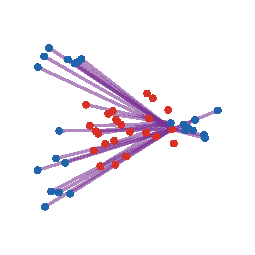
\includegraphics[width=.225\linewidth]{figures/sinkhorn-plan-epsilon/eps-0p008.pdf} &
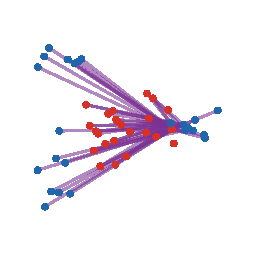
\includegraphics[width=.225\linewidth]{figures/sinkhorn-plan-epsilon/eps-0p025.pdf} &
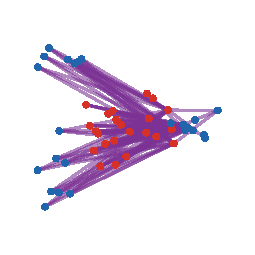
\includegraphics[width=.225\linewidth]{figures/sinkhorn-plan-epsilon/eps-0p080.pdf} &
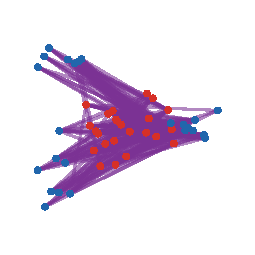
\includegraphics[width=.225\linewidth]{figures/sinkhorn-plan-epsilon/eps-0p250.pdf}
\end{tabular}
\caption{Entropically regularized couplings between the canonical red and blue point clouds for four fixed regularization strengths. The squared Euclidean cost is normalized by its median. Violet segments display the largest visible entries of the computed Sinkhorn plan, with thickness and opacity proportional to transported mass. The computed plans are strictly positive for every $\epsilon>0$, but the visible mass pattern evolves from nearly sparse to diffuse as $\epsilon$ increases.}
\label{fig:sinkhorn-plan-epsilon}
\end{figure}

%%%%%%%%%%%%%%%%%%%%%%%%%%%%%%%%%%%%%%%%%%%%%%%%%%%%%%%%%%%%%%%%%%%%%%%%%%%
\subsection{General Formulation}


The continuous entropic problem is the static Schr\"odinger problem. It gives a probabilistic interpretation of Sinkhorn as the most likely coupling under a noisy reference dynamics.

One can consider arbitrary measures by replacing the discrete entropy with the relative entropy with respect to the product measure $\d\al\otimes\d\be(x,y) \eqdef \d\al(x)\d\be(y)$, and propose a regularized counterpart to~\eqref{eq-mk-generic} using
\eql{\label{eq-entropic-generic}
	\MK_\c^\epsilon(\al,\be) \eqdef
	\umin{\pi \in \Couplings(\al,\be)}
		\int_{\X \times \Y} c(x,y) \d\pi(x,y) + \epsilon \KL(\pi|\al\otimes\be)
}
where the relative entropy is a generalization of the discrete Kullback-Leibler divergence~\eqref{eq-kl-defn}
\eql{\label{eq-defn-rel-entropy}
	\KL(\pi|\xi) \eqdef \int_{\X \times \Y} \log\Big( \frac{\d \pi}{\d\xi}(x,y) \Big) \d\pi(x,y)
	  + \int_{\X \times \Y} (\d\xi(x,y)-\d\pi(x,y)),
}
and by convention $\KL(\pi|\xi)=+\infty$ if $\pi$ does not have a density $\frac{\d \pi}{\d\xi}$ with respect to $\xi$.
%
It is important to realize that the reference measure $\al\otimes\be$ chosen in~\eqref{eq-entropic-generic} to define the entropic regularizing term $\KL(\cdot|\al\otimes\be)$ plays no specific role (because Proposition~\ref{prop-kl-shift} still applies in this general setting), only its support matters.
%
This problem is often referred to as the ``static Schr\"odinger problem'', since $\pi$ is intended to model the most likely coupling between gas particles observed only at two different times (the so-called lazy gas model). The parameter $\epsilon$ controls the temperature of the gas, and particles do not move in a deterministic straight line as in optimal transport for the Euclidean cost, but rather according to a stochastic Brownian bridge. This viewpoint goes back to Schr\"odinger's reciprocal problem~\cite{Schroedinger31} and is surveyed in modern OT language in~\cite{leonard2012schrodinger,LeonardSchroedinger}; stochastic-control formulations are developed in~\cite{chen2016relation}.

\begin{rem}[Probabilistic interpretation]
	If $(X,Y) \sim \pi$ have marginals $X \sim \al$ and $Y \sim \be$, then $\KL(\pi|\al \otimes \be) = \Ii(X,Y)$ is the mutual information of the couple, which is 0 if and only if $X$ and $Y$ are independent. The entropic problem~\eqref{eq-entropic-generic} is thus equivalent to
	\eq{
		\umin{(X,Y), X \sim \al, Y \sim \be } \EE( c(X,Y)) + \epsilon \Ii(X,Y).
	}
	Using a large $\epsilon$ thus enforces the optimal coupling to describe independent variables, while, according to Brenier's theorem, small $\epsilon$ rather imposes a deterministic dependency between the couple according to a Monge map.
\end{rem}


%%%%%%%%%%%%%%%%%%%%%%%%%%%%%%%%%%%%%%%%%%%%%%%%%%%%%%%%%%%%%%%%%%%%%%%%%%%
\subsection{Bregman Projection View of Sinkhorn}
\label{sec-convergence-init}

This subsection explains Sinkhorn as alternating Bregman projections. The main message is geometric: each row or column rescaling is the KL projection onto one affine marginal constraint, so convergence follows from the Pythagorean identity for Bregman divergences.

For the sake of simplicity, this section is written for discrete measures, but the analysis carries over to general measures. This analysis is revisited in Section~\ref{sec-convergence-dual} using convex duality.

%%%%
\paragraph{Alternating $\KL$ projections.}

The projection viewpoint explains Sinkhorn as repeated enforcement of one marginal constraint at a time. It is not specific to the entropy, although the KL case is the one where the projections reduce to elementary row and column scalings.

\begin{defn}[Bregman divergence]\label{def-bregman-divergence}
	Let $\Phi$ be a differentiable strictly convex function on a convex domain $\Omega$. The Bregman divergence generated by $\Phi$ is
	\[
		D_\Phi(P|Q)\eqdef \Phi(P)-\Phi(Q)-\dotp{\nabla\Phi(Q)}{P-Q}.
	\]
	For the negative entropy $\Phi(P)=\sum_{i,j}P_{i,j}\log P_{i,j}$ on the positive orthant, one obtains $D_\Phi(P|Q)=\KLD(P|Q)$ up to the harmless convention at the boundary.
\end{defn}

The main interest of Bregman divergences is that the geometry can encode constraints. A Legendre-type generator $\Phi$ blows up, or has an infinite derivative, at the boundary of its domain; for negative entropy this means that positivity is built into the divergence, so one projects onto affine marginal constraints without separately handling non-negativity.

\paragraph{Linear tilts and Gibbs references.}

The following proposition explains why adding a linear cost to a Bregman penalty merely shifts the reference point in dual coordinates. The usual Gibbs--KL reformulation is the entropy specialization.

\begin{prop}[Linear tilts of Bregman penalties]\label{prop-bregman-linear-tilt}
	Let $\Phi$ be differentiable and strictly convex, and let $D_\Phi$ be its Bregman divergence. Fix a reference point $\Q$ in the interior of the domain. Assume that there exists $\Q^\C$ such that
	\[
		\nabla\Phi(\Q^\C)=\nabla\Phi(\Q)-\C/\epsilon .
	\]
	Then, for all $\P$ in the domain,
	\[
		\dotp{\P}{\C}+\epsilon D_\Phi(\P|\Q)
		=
		\epsilon D_\Phi(\P|\Q^\C)+\text{\upshape cst},
	\]
	where the constant does not depend on $\P$.
\end{prop}
\begin{proof}
	Subtract the two Bregman divergences:
	\[
		D_\Phi(\P|\Q^\C)-D_\Phi(\P|\Q)
		=
		\dotp{\nabla\Phi(\Q)-\nabla\Phi(\Q^\C)}{\P}
		+\text{cst}.
	\]
	Using $\nabla\Phi(\Q)-\nabla\Phi(\Q^\C)=\C/\epsilon$ and multiplying by $\epsilon$ gives the claim.
\end{proof}

For the negative entropy $\Phi(\P)=\sum_{i,j}\P_{i,j}\log\P_{i,j}$, one has $D_\Phi=\KLD$. Taking $\Q=\a\otimes\b$ gives the tilted reference
\[
	\K_{\a,\b}^\epsilon
	\eqdef
	(\a\otimes\b)\odot e^{-\C/\epsilon}.
\]
Thus
\[
	\dotp{\P}{\C}+\epsilon\KLD(\P|\a\otimes\b)
	=
	\epsilon\KLD(\P|\K_{\a,\b}^\epsilon)+\text{\upshape cst}.
\]
On the transport polytope, scaling $\K_{\a,\b}^\epsilon$ is equivalent to scaling the Gibbs kernel $\K=e^{-\C/\epsilon}$ because the factors $\a_i$ and $\b_j$ can be absorbed into the Sinkhorn scalings.

This shows that the unique solution $\P_\epsilon$ of~\eqref{eq-regularized-discr} is a projection onto $\CouplingsD(\a,\b)$ of the tilted Gibbs reference
\eql{\label{eq-kl-proj}
	\P_\epsilon = \Proj_{\CouplingsD(\a,\b)}^\KLD(\K_{\a,\b}^\epsilon) \eqdef \uargmin{\P \in \CouplingsD(\a,\b)} \KLD(\P|\K_{\a,\b}^\epsilon).
}

\paragraph{Cyclic projection convergence.}

The general convergence mechanism is the classical one of Bregman~\cite{bregman1967relaxation}.

\begin{prop}[Cyclic Bregman projections on affine constraints]\label{prop-cyclic-kl-affine}
	Let $\Phi$ be a Legendre strictly convex generator on a finite-dimensional convex domain, and let $\Cc_1,\Cc_2$ be affine constraint sets whose intersection meets the domain. Define
	\[
		P_{k+1}
		=
		\Proj_{\Cc_2}^{D_\Phi}
		\Proj_{\Cc_1}^{D_\Phi}(P_k),
	\]
	starting from an interior point $P_0$, and assume the projections are well-defined. Then $P_k$ converges to the Bregman projection of $P_0$ onto $\Cc_1\cap\Cc_2$. In particular, the KL case converges for positive affine marginal constraints.
\end{prop}
\begin{proof}
	We first prove the Pythagorean identity used by the projection argument. For three interior points one has the Bregman three-point formula
	\[
		D_\Phi(Q|P)
		=
		D_\Phi(Q|P^+)
		+
		D_\Phi(P^+|P)
		+
		\dotp{\nabla\Phi(P^+)-\nabla\Phi(P)}{Q-P^+}.
	\]
	If $P^+=\Proj_\Cc^{D_\Phi}(P)$ and $\Cc$ is affine, the first-order optimality condition for minimizing $R\mapsto D_\Phi(R|P)$ over $R\in\Cc$ is
	\[
		\dotp{\nabla\Phi(P^+)-\nabla\Phi(P)}{R-P^+}=0
		\qquad \forall R\in\Cc,
	\]
	because $R-P^+$ ranges over the tangent linear space of $\Cc$. Taking $R=Q\in\Cc$ cancels the last term and gives
	\[
		D_\Phi(Q|P)=D_\Phi(Q|P^+)+D_\Phi(P^+|P)
		\qquad\forall Q\in\Cc.
	\]

	Let $(Z_\ell)_\ell$ be the half-step sequence obtained by alternating projections onto $\Cc_1$ and $\Cc_2$, so that $Z_{2k}=P_k$ and $Z_{2k+2}=P_{k+1}$. Fix $Q\in\Cc_1\cap\Cc_2$. Applying the identity at each half-step gives
	\[
		D_\Phi(Q|Z_\ell)-D_\Phi(Q|Z_{\ell+1})
		=
		D_\Phi(Z_{\ell+1}|Z_\ell)\geq0.
	\]
	Thus $D_\Phi(Q|Z_\ell)$ is decreasing and the series $\sum_\ell D_\Phi(Z_{\ell+1}|Z_\ell)$ is finite. In finite dimension, the iterates remain in the Bregman sublevel set $\{Z:D_\Phi(Q|Z)\leq D_\Phi(Q|Z_0)\}$; for a Legendre generator this set stays in the domain and is compact under the stated well-definedness assumptions. Hence cluster points exist. Since the projection drops tend to zero and $\Phi$ is strictly convex on compact subsets of the domain, $\norm{Z_{\ell+1}-Z_\ell}\to0$. Every cluster point of the even subsequence is therefore also a cluster point of the adjacent odd subsequence, and because these two subsequences lie alternately in the closed affine sets $\Cc_1$ and $\Cc_2$, every cluster point belongs to $\Cc_1\cap\Cc_2$.

	Let $\bar P$ be such a cluster point. For each half-step, the dual displacement
	\[
		\nabla\Phi(Z_{\ell+1})-\nabla\Phi(Z_\ell)
	\]
	belongs to the normal space of the affine set onto which one projects. Telescoping and using the convergence of $Z_\ell$ gives
	\[
		\nabla\Phi(\bar P)-\nabla\Phi(P_0)
		\in
		N_{\Cc_1}+N_{\Cc_2}
		=
		N_{\Cc_1\cap\Cc_2},
	\]
	where the last equality uses that the sets are affine. This is precisely the first-order optimality condition for minimizing $R\mapsto D_\Phi(R|P_0)$ over $R\in\Cc_1\cap\Cc_2$. Thus $\bar P$ is the Bregman projection of $P_0$ onto the intersection. Strict convexity gives uniqueness of this minimizer, hence all cluster points coincide and the whole sequence converges. The KL statement is obtained by choosing the negative entropy generator.
\end{proof}

Denoting
\eq{
	\Cc^1_\a \eqdef \enscond{\P}{\P\ones_m=\a}
	\qandq
	\Cc^2_\b \eqdef \enscond{\P}{\transp{\P}\ones_n=\b}
}
the rows and columns constraints, one has $\CouplingsD(\a,\b) = \Cc^1_\a \cap \Cc^2_\b$. One can use KL, or more generally Bregman, iterative projections~\cite{bregman1967relaxation,Ruschendorf95,RuschendorfThomsen}
\eql{\label{eq-kl-sinkh-proj}
	\itt{\P} \eqdef \Proj_{\Cc^1_\a}^{\KLD}(\it{\P})
	\qandq
	\ittt{\P} \eqdef \Proj_{\Cc^2_\b}^{\KLD}(\itt{\P}).
}
Since the sets $\Cc^1_\a$ and $\Cc^2_\b$ are affine, Proposition~\ref{prop-cyclic-kl-affine} applies with $P_0=\K_{\a,\b}^\epsilon$ and shows convergence to the solution of~\eqref{eq-kl-proj}.

\paragraph{Row and column scalings.}

The two projectors are simple to compute since they correspond to scaling respectively the rows and the columns, as explained in this proposition.

\begin{prop}[KL projections are scalings]
One has
\eq{
	 \Proj_{\Cc^1_\a}^{\KLD}(\P) = \diag\pa{\frac{\a}{\P \ones_m}} \P
	 \qandq
	 \Proj_{\Cc^2_\b}^{\KLD}(\P) =  \P \diag\pa{\frac{\b}{\P^\top \ones_n}}.
}
\end{prop}
\begin{proof}
	Consider the problem along each row or column vector to impose a fixed sum $s \in \RR_+$
	\eq{
		\umin{p} \enscond{ \KL(p|q) }{ \dotp{p}{\ones}=s }.
	}
	The Lagrange multiplier equation for this problem reads
	\eq{
		\log(p/q)+\la \ones=0 \qarrq
		p = u q \qwhereq u = e^{-\la}>0.
	}
	The constraint $\dotp{p}{\ones} = s$ is equivalent to $\dotp{uq}{\ones}=s$, i.e. $u=s/\sum_i q_i$, which gives the desired scaling formula
	$p=s q/\sum_i q_i$.
\end{proof}

These iterations are equivalent to Sinkhorn iterations~\eqref{eq-sinkhorn} since defining
\eq{\label{eq-sink-matrix}\P^{(2\ell)} \eqdef \diag(\it{\uD}) \K \diag(\it{\vD}),}
one has
\begin{align*}
	\P^{(2\ell+1)} &\eqdef \diag(\itt{\uD}) \K \diag(\it{\vD}) \\
	\qandq
	\P^{(2\ell+2)} &\eqdef \diag(\itt{\uD}) \K \diag(\itt{\vD})
\end{align*}
In practice, however, one should prefer using~\eqref{eq-sinkhorn}, which only requires manipulating scaling vectors and multiplying by a Gibbs kernel, and can often be accelerated when the kernel has separable, sparse, low-rank or geometric structure.

Such a convergence analysis using Bregman projection is of limited interest because it only works in finite dimension. For instance, the linear convergence speed one can obtain with these analyses (because the objective is strongly convex) degrades with the dimension and with $\epsilon$. Section~\ref{sec-convergence-dual} gives a more robust dual analysis: the constants are expressed through the oscillation of the potentials and the cost range, and the resulting $O(1/k)$ estimate explains what can be guaranteed before any asymptotic linear regime becomes visible.
%
It is also possible to decay $\epsilon$ during the iterates to improve the speed and rely on multiscale strategies in low dimensions.


\subsection{Hilbert Metric View of Sinkhorn}
\label{sec-sinkhorn-hilbert}

Hilbert's projective metric gives a complementary convergence mechanism. Instead of following objective values, it measures distances between positive scaling vectors modulo global multiplication. Positive kernels are contractions in this geometry, yielding a global linear convergence statement.

As initially explained by~\cite{franklin1989scaling}, the global convergence analysis of Sinkhorn is greatly simplified using Hilbert projective metric on $\RR_{+,*}^n$ (positive vectors), defined as
\eql{\label{eq-hilbert-metric}
	\foralls (\uD,\uD') \in (\RR_{+,*}^n)^2, \quad
	\Hilbert(\uD,\uD') \eqdef
		\norm{\log(\uD)-\log(\uD')}_V
}
where the variation semi-norm is
\eq{
	\norm{z}_V = \max(z)-\min(z).
}

\begin{prop}[Hilbert metric on the projective cone]
	The function $\Hilbert$ defines a complete distance on the projective cone $\RR_{+,*}^n/\sim$, where $\uD \sim \uD'$ means that $\uD=s\uD'$ for some $s>0$.
\end{prop}
\begin{proof}
	The map $\uD \mapsto \log \uD$ identifies $\RR_{+,*}^n/\sim$ with the quotient vector space $\RR^n/\Span(\ones_n)$, because multiplying $\uD$ by $s>0$ adds the constant vector $\log(s)\ones_n$. The variation semi-norm $\norm{z}_V=\max_i z_i-\min_i z_i$ vanishes exactly on constant vectors, so it induces a norm on this quotient. Symmetry, the triangle inequality and separation therefore follow from the corresponding norm properties. Completeness follows because $\RR^n/\Span(\ones_n)$ is finite-dimensional and all finite-dimensional normed spaces are complete.
\end{proof}
%
It was introduced independently by~\cite{birkhoff1957extensions} and~\cite{samelson1957perron} to provide quantitative proofs of the Perron-Frobenius theorem (convergence of iterations of positive matrices). Sinkhorn should be viewed as a nonlinear generalization of Perron-Frobenius.


\begin{thm}[Birkhoff contraction theorem]\label{thm-birkhoff}
	Let $\K \in \RR_{+,*}^{n \times m}$, then for $(\vD,\vD') \in (\RR_{+,*}^m)^2$
	\eq{
		\Hilbert(\K \vD,\K \vD') \leq \la(\K) \Hilbert(\vD,\vD')
		\text{ where }
		\choice{
			\la(\K) \eqdef \frac{ \sqrt{\eta(\K)}-1 }{ \sqrt{\eta(\K)}+1 } < 1 \\
			\eta(\K) \eqdef \umax{i,j,k,\ell} \frac{ \K_{i,k} \K_{j,\ell} }{ \K_{j,k} \K_{i,\ell} }.
		}
	}
\end{thm}
\begin{proof}
	We recall the finite-dimensional Birkhoff--Hopf estimate. For a positive linear map $A$ on a cone, define its projective diameter
	\[
		\Delta(A) \eqdef \sup_{u,v>0} \Hilbert(Au,Av).
	\]
	Then
	\[
		\Hilbert(Au,Av) \leq \tanh(\Delta(A)/4)\Hilbert(u,v).
	\]
	Indeed, after quotienting by positive scalings, write $r_k=u_k/v_k$ and normalize so that $e^{-h/2}\leq r_k\leq e^{h/2}$, where $h=\Hilbert(u,v)$. The ratio between two coordinates of $Au/Av$ is a quotient of two weighted averages of the numbers $r_k$. A two-point extremal argument shows that the largest possible contraction is obtained when the mass of the two weights is placed on the two endpoints $e^{-h/2}$ and $e^{h/2}$; the cross-ratio bound defining $\Delta(A)$ then gives
	\[
		\Hilbert(Au,Av)
		\leq
		2\log\frac{e^{\Delta(A)/4}e^{h/2}+e^{-\Delta(A)/4}e^{-h/2}}
		{e^{\Delta(A)/4}e^{-h/2}+e^{-\Delta(A)/4}e^{h/2}}
		\leq \tanh(\Delta(A)/4)h.
	\]
	For the matrix $\K$, its projective diameter is
	\[
		\Delta(\K)=\log \eta(\K),
		\qquad
		\eta(\K)=\max_{i,j,k,\ell}
		\frac{\K_{i,k}\K_{j,\ell}}{\K_{j,k}\K_{i,\ell}}.
	\]
	Therefore $\tanh(\Delta(\K)/4)=(\sqrt{\eta(\K)}-1)/(\sqrt{\eta(\K)}+1)$, which is the claimed contraction factor.
\end{proof}

This result extends to arbitrary convex cones and affine mappings from the cone to its interior.

The following theorem proved by~\cite{franklin1989scaling}, makes use of this Theorem~\ref{thm-birkhoff} to show the linear convergence of Sinkhorn's iterations.

\begin{thm}[Linear convergence of Sinkhorn]
	One has $(\it{\uD},\it{\vD}) \rightarrow (\uD^\star,\vD^\star)$ and
	\eql{\label{eq-convlin-sinkh}
		\Hilbert(\it{\uD}, \uD^\star) = O(\la(\K)^{2\ell}), \quad
		\Hilbert(\it{\vD}, \vD^\star) = O(\la(\K)^{2\ell}).
	}
	One also has
	\eql{\label{eq-convsinkh-control}
		\Hilbert(\it{\uD}, \uD^\star) \leq \frac{\Hilbert( \it{\P}\ones_m,\a )}{1-\la(\K)}
		\qandq
		\Hilbert(\it{\vD}, \vD^\star) \leq \frac{\Hilbert( \P^{(\ell),\top} \ones_n,\b )}{1-\la(\K)},
	}
	where we denoted $\it{\P} \eqdef \diag(\it{\uD}) \K \diag(\it{\vD})$. Lastly, one has
	\eql{\label{eq-convlin-sinkh-prim}
		\norm{\log(\it{\P}) - \log(\P^\star)}_\infty \leq \Hilbert(\it{\uD}, \uD^\star) + \Hilbert(\it{\vD}, \vD^\star)
	}
	where $\P^\star$ is the unique solution of~\eqref{eq-regularized-discr}.
\end{thm}

\begin{proof}
	Notice that for any $(\vD,\vD') \in (\RR_{+,*}^m)^2$, one has
	\eq{
		\Hilbert(\vD,\vD') = \Hilbert(\vD/\vD',\ones_m) = \Hilbert(\ones_m/\vD,\ones_m/\vD'),
	}
	since indeed $\Hilbert(\a/\vD,\a/\vD') = \Hilbert(\vD,\vD')$.
	%
	This shows that
	\begin{align*}
		\Hilbert(\itt{\uD},\uD^\star) &= \Hilbert\pa{ \frac{\a}{\K \it{\vD}}, \frac{\a}{\K \vD^\star} }
		= \Hilbert( \K \it{\vD}, \K \vD^\star ) \leq \la(\K) \Hilbert( \it{\vD}, \vD^\star ).
	\end{align*}
	where we used Theorem~\ref{thm-birkhoff}. This shows~\eqref{eq-convlin-sinkh}.  One also has, using the triangular inequality
	\begin{align*}
		\Hilbert(\it{\uD},\uD^\star) &\leq \Hilbert(\itt{\uD},\it{\uD}) + \Hilbert(\itt{\uD},\uD^\star)
		\leq \Hilbert\pa{ \frac{\a}{\K \it{\vD}},\it{\uD} } + \la(\K) \Hilbert(\it{\uD},\uD^\star) \\
		&= \Hilbert\pa{ \a,\it{\uD} \odot  ( \K \it{\vD} ) } + \la(\K) \Hilbert(\it{\uD},\uD^\star),
	\end{align*}
	which gives the first part of~\eqref{eq-convsinkh-control} since
	$\it{\uD} \odot  ( \K \it{\vD} ) = \it{\P}\ones_m$ (the second one being similar).
	%
	The proof of~\eqref{eq-convlin-sinkh-prim} follows from~\cite[Lemma 3]{franklin1989scaling}
\end{proof}

The bound~\eqref{eq-convsinkh-control} shows that some error measures on the marginal constraints violation, for instance, $\norm{\it{\P} \ones_m - \a}_1$ and $\norm{\transp{\it{\P}} \ones_n - \b}_1$, are useful stopping criteria to monitor the convergence.
This theorem shows that the Sinkhorn algorithm converges linearly, but the worst-case rate becomes exponentially bad as $\epsilon \rightarrow 0$, since the global contraction factor is controlled by a term of the form $e^{-\norm{c}_\infty/\epsilon}$. In practice, one often observes a much better local linear regime after enough iterations.
%
The same Hilbert-metric mechanism extends beyond finite matrices to positive integral operators under suitable compactness and positivity assumptions.
%
An important limitation of this analysis is that it requires a uniformly bounded cost and a kernel bounded away from degeneracy; Gaussian distributions with quadratic cost therefore require a different approach.
